 
\begin{figure}[htbn]
\begin{center}
\noindent    
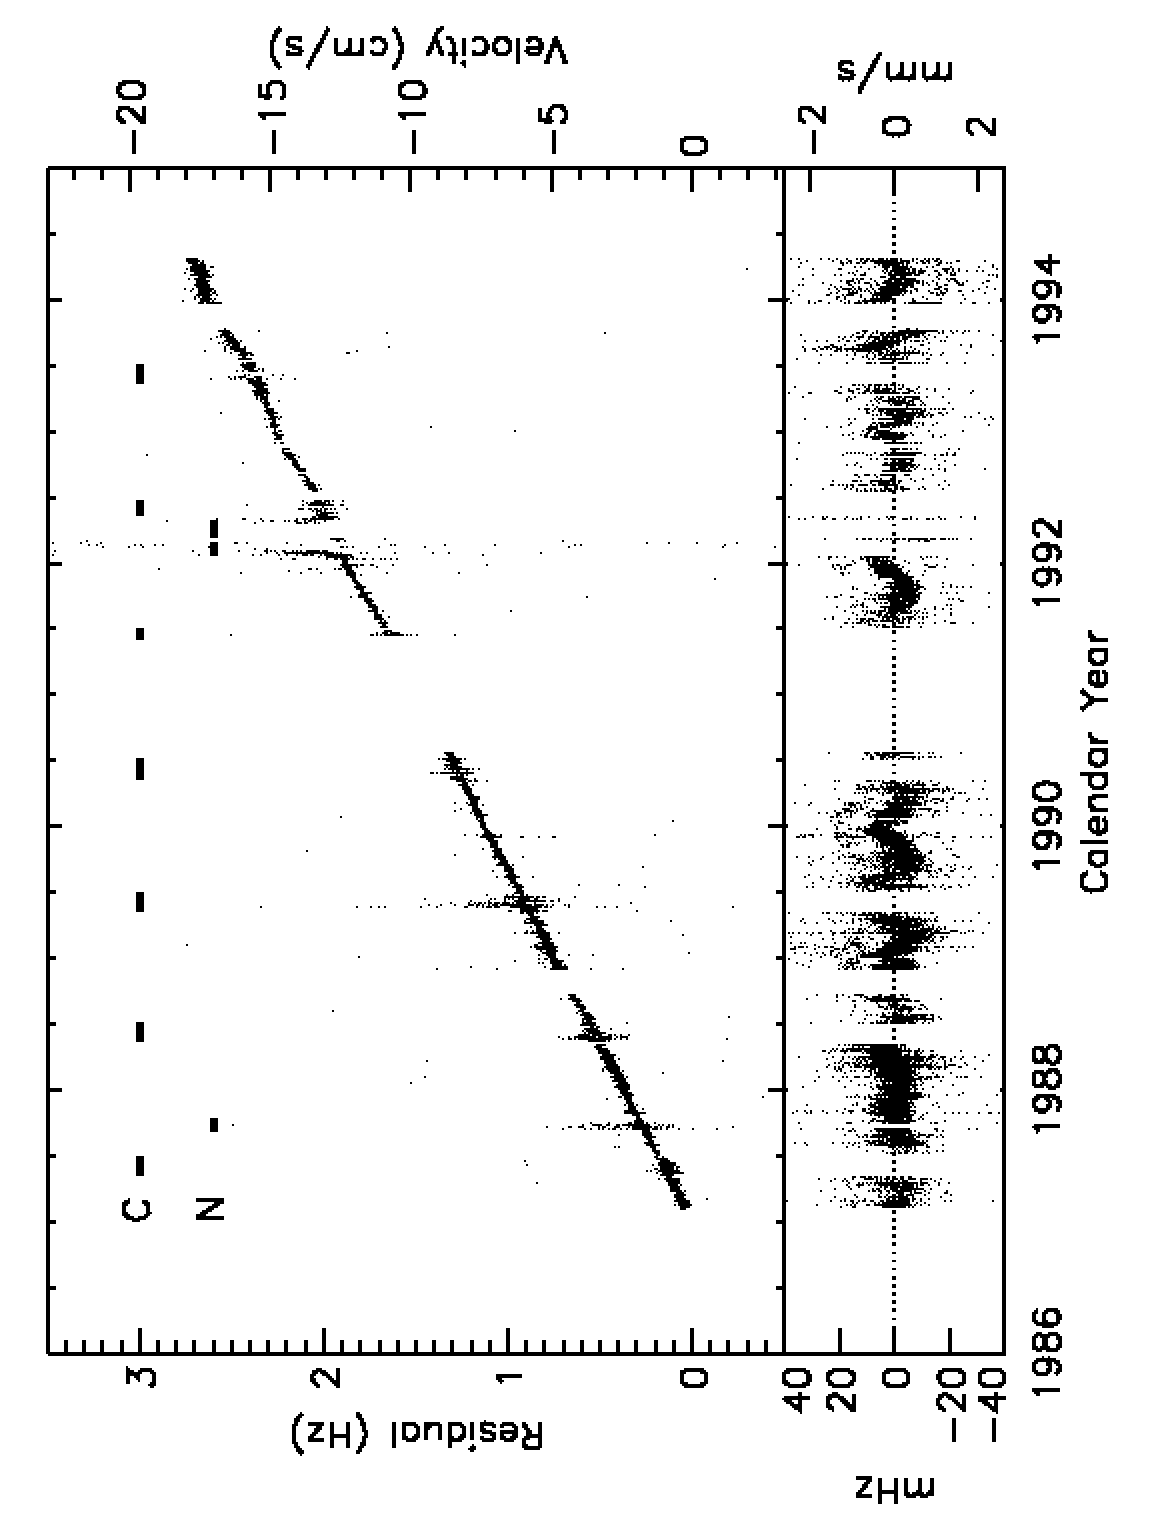
\includegraphics[angle=-90,width=0.8\linewidth]{images/M02P10beide}
\end{center}
\vskip -10pt
  \caption{Die Abweichungen von der Vorhergesagten Bahn. {\bf Oben:} ohne Berücksichtigung einer Anomalie; {\bf Unten:} mit Berücksichtigung der Anomalie. Die Beiden mit C und N markierten Zeilen oben, zeigen Zeiten an in welchen die Daten von der Auswertung ausgeschlossen wurden, weil die Daten durch Effekte Sonnen corona (C) beziehungsweise unbekannte Gründe (N) stark verrauscht waren. Es handelt bei diesem Bild um das Ergebnis von Markwardts Analyse\cite{Markwardt2002}.}\label{fig:Markwardvergl}
\end{figure} 
 
\begin{figure}[htnb]
\begin{center}
\noindent    
\psfig{figure=images/correlated,width=\linewidth,height=\textheight,keepaspectratio}
\end{center}
\vskip -10pt
  \caption{
Verlauf der anomalen Beschleunigung in Abhängigkeit von der Entfernung in Astronomischen Einheiten. Diese Tabelle zeigt das Resultat einer groben Auswertung der Daten an, sie ist noch kein Ergebnis der in Arbeit befindlichen, genauen Analyse der Daten über den gesamten Zeitraum. Die Ersterscheinung dieser Grafik konnte nicht ermittelt werden, sie taucht jedoch in zahlreichen Arbeiten auf, darunter\cite{Anderson2002}\cite{Nieto2005}\cite{Turyshev2010}
}
\label{fig:anomalie}
\end{figure} 
 
\subsection{Die Anomalie}
Geht man nun davon aus, dass unsere physikalischen Modelle richtig sind und wir alle relevanten Einflüsse berücksichtigt haben, so erwartet man im Rahmen der Messgenauigkeit für $a_P = 0$ eine Übereinstimmung im Fit.
Zunächst schien dies auch noch der Fall zu sein, nach dem Flyby-Manöver am Saturn im Jahr 1979 änderte sich dies für Pioneer 11 aber deutlich. Zu diesem Zeitpunkt befand sich die Sonde in einer Entfernung von etwa 20 AU und somit war die Beschleunigung durch den, in niedrigen Entfernungen nur ungenau berechenbaren, solaren Strahlungsdruck auf unter $5 \cdot 10^{-8} \frac{cm}{s^2}$ gesunken,
somit sank auch die Messungenauigkeit weit genug, um das nun zu Tage tretende Phänomen nicht mehr länger zu verschleiern.
Auch für Pioneer 10 stellte man bald darauf eine Abweichung fest.

Die Analyse der Daten von 1987 bis 1998 – das entspricht solaren Entfernungen von 20 bis 70 AU –
zeigte eine zeitlich konstant zunehmende anomale Blauverschiebung von
\begin{equation}
  \frac{d\Delta\nu}{dt}=(5,99\pm0,01)\cdot10^{-9}\frac{Hz}{s}
\end{equation}
wobei $\Delta\nu=[\nu_{Messung}-\nu_{Modell}]'_E$ ist\cite{Dittus2006}. Der Fehler hierbei ist nur der statistische Fehler. Die zunehmende Blauverschiebung ist im oberen Teil von Abbildung~\ref{fig:Markwardvergl} deutlich zu sehen. Lässt man die Software, die Bahn ohne eine Anomalie an die Werte fitten, so versucht sie  die Kurve durch Manöver anzupassen – man erhält dabei jedoch starke Abweichungen, weshalb ein solches Modell auszuschließen ist\cite{Markwardt2002}.

Lässt man, wie oben beschrieben, beim Fitten eine zusätzliche Beschleunigung zu, so erhält man eine wesentlich bessere Übereinstimmung (siehe Abbildung \ref{fig:Markwardvergl}, unten). Die dabei gefundenen Werte der Anomalie für die beiden Sonden sind:
\begin{eqnarray}
  a_{Pioneer 10} = (7,84\pm0,01)\cdot10^{-8}\frac{cm}{s^2} \\  
  a_{Pioneer 11} = (8,55\pm0,02)\cdot10^{-8}\frac{cm}{s^2}
\end{eqnarray}

Zwischen den obigen Werten lässt sich aus Gleichung (\ref{equ:rel}) ein direkter physikalischer Zusammenhang ableiten. Verwendet man die vereinfachte Version (\ref{equ:einf_rel}), so erhält man:
\begin{equation}
  a_{Pioneer}=\frac{dv}{dt}=\frac{1}{2}\frac{c}{\nu_E}\frac{d\Delta\nu}{dt}
\end{equation}
%oder
%\begin{equation}
%  \Delta\nu=-\nu_E \frac{2a_p t}{c}
%\end{equation}

Berücksichtigt man den Einfluss aller bekannter Effekte auf den Wert und die Unsicherheit der Größe\cite{Turyshev2004}, so erhält man einen endgültige Wert von:  
\begin{equation}
  a_{Pioneer} = (8,74\pm1,33)\cdot10^{-8}\frac{cm}{s^2}
\end{equation}

Andere Arbeiten mit den  unterschiedlichen Orbit Determination Codecs bestimmten die Beschleunigung zu $(7,70
\pm0,02)\cdot10^{-8}\frac{cm}{s^2}$ (Markwardt, 2002)\cite{Markwardt2002} beziehungsweise % anderen Wert von Markward
$(8,4\pm0,1)\cdot10^{-8}\frac{cm}{s^2}$ (Levy et al., 2008)\cite{Levy2008}.
Wobei beide Arbeiten sich nur auf Pioneer 10 beziehen und jeweils nur die statistischen Fehler angeben.
Wir wollen uns im folgenden jedoch – wie auch praktisch jede Arbeit der Fachliteratur – auf den oben angegebenen von
Anderson et al. berechneten Wert beschränken.
%% wohin damit:
% Die Standartabweichung bei einem Fit mit dieser konstanten Beschleunigung ist deutlich kleiner als ohne. % 9,8 mHz bei Levy

Der Wert mag zwar klein erscheinen, doch ist seine Größenordnung nur das $10^{-5}$ fache der Newtonschen Beschleunigung,
und er ist größer als die Faktoren $U/c^2$,$v^2/c^2$,$r a/c^2$ zur relativistischen Korrektur der newtonschen Dynamik.
% richtig?
Seit 1979 ist die Sonde um fast eine halbe Million Kilometer von der berechneten Bahn abgewichen:
\begin{equation}
  \Delta x= \frac12 \cdot a_p \cdot (2011-1979)^2 a^2\approx 445.000 km
\end{equation}

Diese Frequenzverschiebung wurde mit nur maximal 3\% Unterschied bei beiden Pioneer-Sonden unabhängig voneinander
gefunden. Das anomale Signal variiert über den analysierten Zeitraum um nur maximal 3,4\%\cite{Turyshev2004}.
Olsen zeigt jedoch, dass es bei der derzeitigen Datenlage nicht auszuschließen ist, dass die Anomalie mit der Zeit abnimmt.\cite{Olsen2006}
Die Richtung der
Beschleunigung ist mit einer Auflösung von 3° bisher noch recht ungenau bestimmt worden. Es ist daher nicht sicher möglich
zu sagen ob die Beschleunigung
in Richtung Sonne, Erde, negativer Geschwindigkeit oder Drehachse geht, dazu mehr in Kapitel XXX.

Eine alternative Interpretation zu einer konstanten Beschleunigung, wäre eine zeitliche Beschleunigung.
So ließe sich die Anomalie auch durch eine zeitliche Beschleunigung von $a_t = (2,92 \pm 0,044) \cdot 10^{-18} s^{-2}$ schreiben.

